%Input premable
\documentclass{beamer}

%Packages
\usepackage{graphicx}
\usepackage{graphics}
\usepackage{hyperref}
\usepackage[english]{babel}
\usepackage{amsmath}
\usepackage{amsfonts}
\usepackage{amssymb}
\usepackage{bm}
\usepackage{etoolbox}
\usepackage{graphicx}
\usepackage{tabularx,ragged2e,booktabs}
\usepackage{caption}
\usepackage{hyphenat}
\usepackage{fixltx2e}
\usepackage[para]{threeparttable}
\usepackage[capposition=top]{floatrow}
\usepackage{subcaption}
\usepackage{pdfpages}
\usepackage{natbib}
\usepackage{rotating}

%Commands
\newcommand\independent{\protect\mathpalette{\protect\independenT}{\perp}}
\def\independenT#1#2{\mathrel{\rlap{$#1#2$}\mkern2mu{#1#2}}}
\newcommand{\overbar}[1]{\mkern 1.5mu\overline{\mkern-1.5mu#1\mkern-1.5mu}\mkern 1.5mu}
\newcommand{\equald}{\ensuremath{\overset{d}{=}}}

\newenvironment{wideitemize}{\itemize\addtolength{\itemsep}{10pt}}{\enditemize}

\mode<presentation>
	{
	\usetheme{UChicagoJorge}
	\setbeamercovered{transparent = 28}
	}

%\usecolortheme{UChicagoJorge} 
%\useinnertheme{UChicagoJorge}
%\useoutertheme{UChicagoJorge}

\title{College Enrollment and Dropout}
\subtitle{Stepping Stone and Option Value}
\author{Econ 350, Jorge L. Garc\'{i}a}
\date{This draft: \today}

\begin{document}


\begin{frame}[plain]
	\titlepage
\end{frame}


\AtBeginSection[]
{
   \begin{frame}
       \frametitle{Outline}
       \tableofcontents[currentsection]
   \end{frame}
}

\section{Ozdagli \& Trachter, 2011}

\begin{frame}
	\frametitle{Paper}
		\begin{itemize}
			\item On the Distribution of College Dropouts: Wealth and Uninsurable Idiosyncratic Risk
			\item 2011
			\item Ali K. Ozdagli (FRB-Boston) and Nicholas Trachter (FRB-Richmond)
			\item R\&R JOLE 
		\end{itemize}
\end{frame}

\begin{frame}
	\frametitle{Overview}
		\begin{itemize}
			\item Dynamic model of the decision to pursue college
				\begin{enumerate}
					\item Students' uncertainty: about future income stream due to unobserved scholastic ability
					\item Expectations reevaluation: on success in college after matriculation and after taking exams 
				\end{enumerate}
			\item Findings (only theoretical)
				\begin{enumerate}
					\item Poorer students are
						\begin{itemize}
							\item less likely to graduate
							\item likely to dropout sooner
						\end{itemize}
				\end{enumerate}
			\item Interesting feature: no need to introduce credit constraints
		\end{itemize}
\end{frame}

\begin{frame}
	\frametitle{Motivation}
		\begin{itemize}
			\item The authors motivate their work claiming that inequality perpetuates and exacerbates as follows:
				\begin{enumerate}
					\item Large fraction of every cohort that enrolls in for year U.S. colleges drops out
			\item High concentration of dropouts among students from lower-income families
			\item Students from low-income families drop out earlier than students from high-income families
			\item Less low-income individuals graduate from college
			\item High return to education
				\end{enumerate}
		\end{itemize}
\end{frame}

\begin{frame}
	\frametitle{Motivation, contd 1}
		\begin{figure}[H] 
		\caption*{}
		\centering
		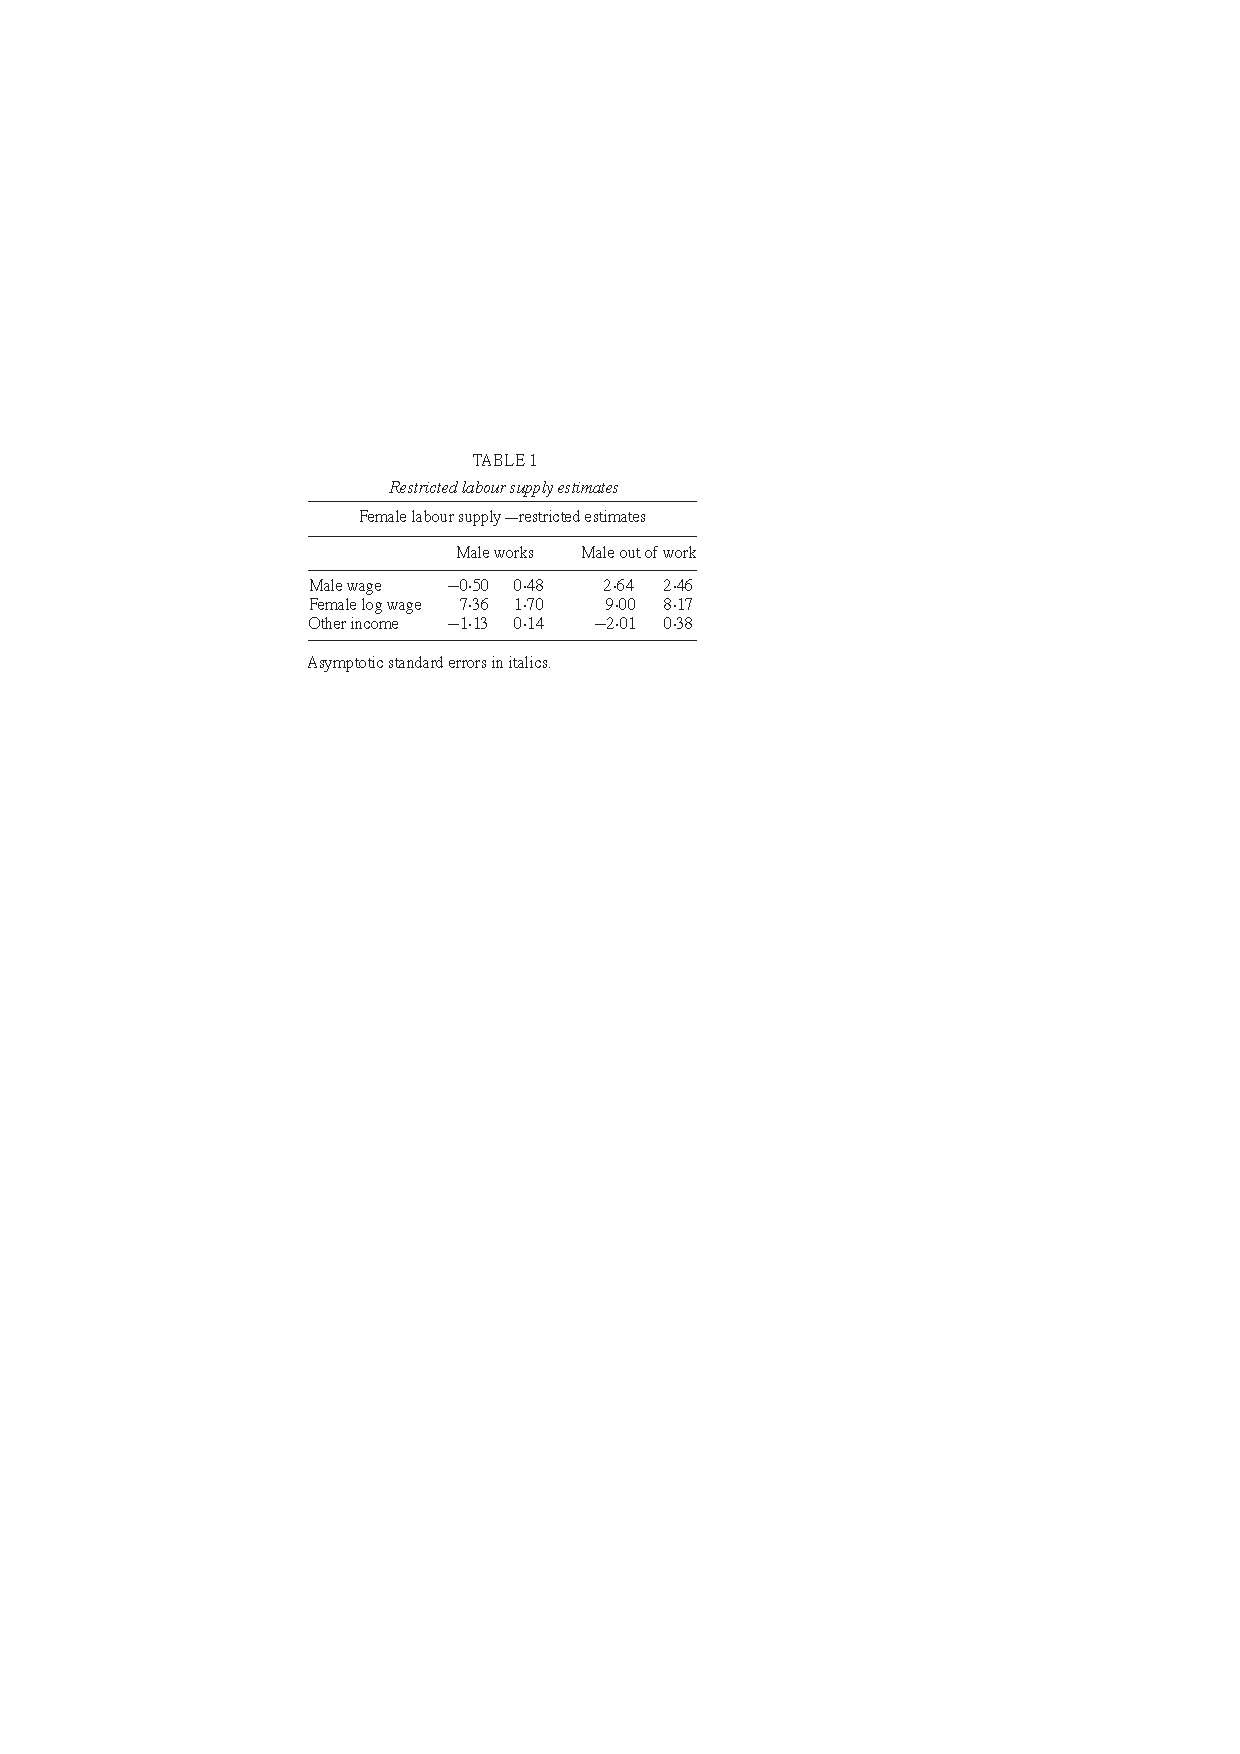
\includegraphics[width=3.5in, height=2in]{Figures/OT/table1.png}
		\end{figure}
\end{frame}

\begin{frame}
	\frametitle{Motivation, contd 2}
		\begin{figure}[H] 
		\caption*{}
		\centering
		\includegraphics[width=3.5in, height=2in]{Figures/OT/table2.png}
		\end{figure}
\end{frame}

\begin{frame}
	\frametitle{Motivation, contd 3}
		\begin{figure}[H] 
		\caption*{}
		\centering
		\includegraphics[width=3.5in, height=2in]{Figures/OT/table3.png}
		\end{figure}
\end{frame}

\begin{frame}
	\frametitle{Motivation, contd 4}
		\begin{figure}[H] 
		\caption*{}
		\centering
		\includegraphics[width=2.5in, height=2.5in]{Figures/OT/figure3.png}
		\end{figure}
\end{frame}

\begin{frame}
	\frametitle{Motivation, contd 5}
		\begin{figure}[H] 
		\caption*{}
		\centering
		\includegraphics[width=2.5in, height=2.5in]{Figures/OT/figure2.png}
		\end{figure}
\end{frame}

\begin{frame}
	\frametitle{Motivation, contd 6}
		\begin{figure}[H] 
		\caption*{}
		\centering
		\includegraphics[width=2.5in, height=2.5in]{Figures/OT/figure1.png}
		\end{figure}
\end{frame}

\begin{frame}
	\frametitle{Model, Basics}
	\begin{itemize}
		\item Based on Miao and Wang (2007): framework of entrepreneurial learning and analysis
		\item Add relevant ingredients of dropout decision:
			\begin{enumerate}
				\item Wage profile: depends on experience and college graduation (and corresponding interaction
				\item Include information unfolding through learning about unobserved ability in college
			\end{enumerate}
	\end{itemize}
\end{frame}

\begin{frame}
	\frametitle{Model, Information}
		\begin{itemize}
			\item The author argues that credit constraints and learning about risk are not fundamental
				\begin{itemize}
					\item Credit constrains: (i) $29\%$ of students from the richest families dropout (NLSY79); (ii) rising house prices lead to higher graduation rates, especially among low-income families (NLSY97)
					\item Learning about stochastic taste: no relation with wealth
				\end{itemize}
		\item Decides to model information unfolding through learning about ability
		\end{itemize}
\end{frame}

\begin{frame}
	\frametitle{Model, Primitives}
		\begin{itemize}
			\item Continuous time, finite horizon; $t \in [0,T]$
			\item At $t=0$
				\begin{enumerate}
					\item Initial endowment, $x(0) \equiv x_{0}$
					\item Unobserved ability to acquire human capital, $\mu \in \{0,1\}$
					\item Prior on ability, $\Pr(\mu = 1 | t = 0) = p(0) \equiv p_{0}$
					\item Either enrolled in college (full-time) or working (in low-skilled or high-skilled sector)
					\item High-skill sector only hires high-skilled workers with college degrees
					\item Work: absorbing state
				\end{enumerate}
					\item Wage function:
						\begin{eqnarray}
							\tilde{w} \left( \mu, \tau \right)
							\begin{cases}
								w(\tau) &,  \tau > 0 \\
								w_{0}    &,  \tau = 0, \mu = 0 \\
								w_{1}   &,  \tau = 0, \mu = 1 
							\end{cases} 
						\end{eqnarray}
\noindent with $\tau = T - t, w_{0} \equiv w(0) < w_{1}$; $\tau_{0} > \tau_{1} \Leftrightarrow w_{1} > w_{0}$. 
		\end{itemize}
\end{frame}

\begin{frame}
	\frametitle{Model, Primitives contd 1}
		\begin{figure}[H] 
		\caption*{Figure 4. Wage Function}
		\centering
		\includegraphics[width=2in, height=1.5in]{Figures/OT/figure4.png}
		\end{figure}
\end{frame}

\begin{frame}
	\frametitle{Model, Primitives contd 2}
		\begin{itemize}
			\item $c$, consumption
			\item $a$, per-unit of time cost of college
			\item $\rho$, discount factor; $r$, interest rate
			\item $\gamma$, CRRA parameter
			\item $\lambda_{1}$, probability of getting an excellent grade for high ability student
			\item $\lambda_{0}$, probability of getting a failing grade for low ability student
				\begin{itemize}
					\item Interpret $\lambda_{1},\lambda_{0}$ as speed of learning
					\item In a continuous (Brownian motion) setting this is analogue to having two volatility parameters
				\end{itemize}
		\end{itemize}
\end{frame}

\begin{frame}
	\frametitle{Model, Primitives contd 2}
		\begin{figure}[H] 
		\caption*{}
		\centering
		\includegraphics[width=2.5in, height=.5in]{Figures/OT/table4.png}
		\end{figure}
\end{frame}

\begin{frame}
	\frametitle{Model, Primitives contd 3}
		\begin{itemize}
			\item Evolution of wealth
				\begin{eqnarray}
					\dot{x} = 
						\begin{cases}
							rx + \tilde{w}(\mu, \tau) - c &, \text{if working} \\
							rx - a - c &, \text{if enrolled in college} \label{eq:x}
						\end{cases}
				\end{eqnarray}
		\end{itemize}
\end{frame}

\begin{frame}
	\frametitle{Model, Student's Problem (Sequential)}
		\begin{equation}
			\max _{ c(t)}\mathbb{E} \left\{ \int \limits _{0} ^{\infty} \exp ^{- \rho t} \frac{c(t)^{1 - \gamma}}{1 - \gamma} | p_{0}, x_{0}  \right\}
		\end{equation}
\noindent s.t. \eqref{eq:x} holds
\end{frame}

\begin{frame}
	\frametitle{Model, Student's Problem (Recursive)}
		\begin{itemize}
			\item $J(x,p,\tau)$, student's with current wealth $x$, prior on ability $p$, $\tau$ time before graduation value function
			\item $V(x,\mu,\tau)$, with current wealth $x$, type $\mu$, $\tau$ time before graduation value function
		\end{itemize}
\end{frame}

\begin{frame}
	\frametitle{Model, Worker's Value Function}
		\begin{itemize}
			\item Instantaneous utility derived: consumption + change in wealth
				\begin{equation}
					\rho V(x,\mu,\tau) = \max_{c} \frac{c^{1 - \gamma}}{1 - \gamma} + V_{x}(x,\mu,\tau)\dot{x}
				\end{equation}
			\item First order condition:
				\begin{equation}
					c^{- \gamma} = V_{x}(\cdot)
				\end{equation}
			\item Define $W(\mu, \tau)$ as the present value of earnings, let $A$ be a constant in terms of $\gamma, \rho$, and rearrange to get
				\begin{equation}
					V(x,\mu,\tau) = A \left( r \left[ x + W(\mu,\tau) \right]  \right)^{1 - \gamma} \label{eq:workers}
				\end{equation}
			\item Note that this implies that the fact that wages are constant is relatively easy to assume away by changing $W(\cdot)$ in \ref{eq:workers}
		\end{itemize}
\end{frame}

\begin{frame}
	\frametitle{Model, Student's Value Function with Known Types}
		\begin{itemize}
			\item Focus on $\mu = 1$ 
			\item For $\mu = 0$ we wait for the results (want to guarantee that $J(x,0,\tau) = V(x,0,\tau)$)
			\item Same principle leads to
				\begin{equation}
					\rho J(x,1,\tau) = \max_{c} \frac{c^{1-\gamma}}{1 - \gamma} + J_{x}(x,1,\tau) \dot{x} + J_{\tau}(x,1,\tau) \dot{\tau}  
				\end{equation}
\noindent with $J(x,1,0) = J(x,1,0)$
			\item First order condition
				\begin{equation}
					c^{1 - \gamma} = J(x,1,\tau) 
				\end{equation}
			\item Solve to get
				\begin{equation}
					J(x,1,\tau) = A \left[ r \left( x + \exp^{r \tau} W(1,0) - a \frac{1 - \exp^{r \tau}}{r} \right) \right]^{1 - \gamma}
				\end{equation}
		\end{itemize}
\end{frame}

\begin{frame}
	\frametitle{\begin{small} Student's Value Function with Unknown Types \end{small}}
	\begin{itemize}
		\item Difficulties
			\begin{enumerate}
				\item Wage upon graduation depends on true ability
				\item New information arrives after each exam
				\item Some students drop out
			\end{enumerate}
		\item Prior's evolution
			\begin{eqnarray}
				p(t+dt) =
					\begin{cases}
						0 &, \text{fails} \\
						1 &, \text{excellent grade} \\
						\frac{p(t) \left[1-\lambda_{1}dt \right]}{p(t) \left[1-\lambda_{1}dt \right] + (1-p(t)) \left[1-\lambda_{0}dt \right]} &, \text{otherwise}
					\end{cases}
			\end{eqnarray}
		\item If the student does not fail or has an excellent grade then
			\begin{equation}
				\dot{p} = - \left( \lambda_{1} - \lambda_{0} \right) p (1 - p)
			\end{equation}
	\end{itemize}		
\end{frame}

\begin{frame}
	\frametitle{Model, Time-line}
		\begin{figure}[H] 
		\caption*{}
		\centering
		\includegraphics[width=2.5in, height=2in]{Figures/OT/figure5.png}
		\end{figure}
\end{frame}

\begin{frame}
	\frametitle{\begin{small} Student's Value Function with Unknown Types, contd 1 \end{small}}
		\begin{itemize}
			\item Same principle leads to		
			\begin{eqnarray}
				\rho J(x,p,\tau) &=& \max_{c} \frac{c^{1- \gamma}}{1- \gamma} + J_{x}(x,p,\tau)\dot{x} + J_{p}(x,p,\tau)\dot{p}  \nonumber \\ 
								 &+& J_{\tau}(x,p,\tau)\dot{\tau} + \lambda_{1} p \left[ J(x,1,\tau) - J(x,p,\tau) \right] \nonumber \\ 
								 &+& \lambda_{0} (1 - p) \left[ V(x,0,\tau) - J(x,p,\tau) \right] 
			\end{eqnarray}
			\item Define $p^*(x,\tau)$ as the threshold such that if $p \leq p^*(x,\tau)$ the student drops out college	
			\end{itemize}		
\end{frame}

\begin{frame}
	\frametitle{\begin{small} Student's Value Function with Unknown Types, contd 1 \end{small}}
		\begin{itemize}
			\item Terminal conditions
				\begin{enumerate}
					\item Terminal Condition
						\begin{equation}
							J(x,p,0) = p V(x,1,0) + (1-p) V(x,0,0) 
						\end{equation}
					\item Value Matching Condition
						\begin{equation}
							J(x,p^*(\cdot),\tau) = V(x,\tau,0)
						\end{equation}
					\item Smooth Pasting Conditions
						\begin{eqnarray}
							J_{p}(x,p^*(\cdot),\tau) &=& 0 \\
							J_{x}(x,p^*(\cdot),\tau) &=& V_{x}(x,\tau,0)\\
							J_{\tau}(x,p^*(\cdot),\tau) &=& V_{\tau}(x,\tau,0)
						\end{eqnarray}
				\end{enumerate}
		\end{itemize}
\end{frame}

\begin{frame}
	\frametitle{\begin{small} Student's Value Function with Unknown Types, contd 2 \end{small}}
		\begin{itemize}
			\item Use FOC to obtain
				\begin{equation}
					p^*(x,\tau) = \frac{a + rW(0,\tau) + W_{\tau} (0,\tau)}{\lambda_{1}} \frac{V_{x}(x,0,\tau)}{J(x,1,\tau) - V(x,0,\tau)}
				\end{equation}
		\end{itemize}
	
\end{frame}

\begin{frame}
	\frametitle{Results, Known Types}
		\begin{itemize}
			\item Lemma 1
				\begin{itemize}
					\item Assume $r \exp^{-r \tau} W(1,0) - a (1 - \exp^{-r \tau})  \geq r W(1, \tau)$
					\item A student of type $\mu = 1$ with current state $(x,\tau)$ chooses to remain in college until $\tau = 0$
					\item Intuition: graduation premium needs to be high enough for high-ability types to remain in college 
				\end{itemize}
			\item Lemma 2
				\begin{itemize}
					\item Assume $a + r W(0,\tau) + W_{\tau} (0,\tau) > 0$	
					\item A student of type $\mu = 0$ immediately drops college
					\item Intuition: if the per-unit marginal cost of attending college is positive, the low-skilled type student drops college immediately
					\item Implication: $J(x,0,\tau) = V(x,0,\tau)$
				\end{itemize}				 
		\end{itemize}
\end{frame}

\begin{frame}
	\frametitle{Results, Unknown Types}
		\begin{itemize}
			\item Result 1
				\begin{itemize}
					\item Let the assumptions in Lemmas 1 and 2 hold
					\item Students with a greater endowment have a lower value of $p^*$, i.e. the belief threshold for which they drop college is lower
					\begin{equation}
						\frac{\partial p^*(x, \tau)}{\partial x} < 0
					\end{equation}
				\end{itemize}
			\item Let $\tau^*$ denote the time to graduation at the moment individual joins the workforce
				\begin{itemize}
					\item $\tau^* = T$, joins workforce immediately
					\item $\tau^* = 0$, joins workforce with college degree
				\end{itemize}
		\end{itemize}
\end{frame}

\begin{frame}
	\frametitle{Results, Unknown Types contd 1}
		\begin{itemize}
			\item Proposition 1
				\begin{itemize}
					\item Consider two endowments $x_{0}^i, x_{0}^j$ with $x_{0}^i > x_{0}^j$
					\begin{equation}
					\forall \ \bar{\tau} \in \mathbb{R}_{++}, \Pr \{ \tau^* \leq \bar{\tau} | x_{0}^i, p_{0}, \mu \} = \Pr \{ \tau^* \leq \bar{\tau} | x_{0}^j, p_{0}, \mu \}
					\end{equation}
					\item Intuition: given a skill level. $\mu$, and a initial belief, $p_{0}$, richer students drop out later (and have longer expected tenures!)
					\item Corollary: once condition on ability type and prior belief richer students are more likely to graduate from college
				\end{itemize}
		\end{itemize}
\end{frame}

\section{Trachter, 2014}

\end{document}